\documentclass[12pt, a4paper]{report}

\usepackage[T2A]{fontenc}
\usepackage[utf8]{inputenc}
\usepackage[english,russian]{babel}
\usepackage[left = 1 cm, right = 1 cm, top = 2cm, bottom = 2 cm, bindingoffset = 0 cm]{geometry}
\usepackage{amsmath,amsfonts,amssymb,amsthm,mathtools}
\usepackage{wasysym}
\usepackage{float}

\usepackage{graphicx}
\graphicspath{{pictures/}}
\DeclareGraphicsExtensions{.pdf,.png,.jpg}

\usepackage{alltt}

\begin{document}
\begin{titlepage}
\newpage

\begin{center}
Министерство образования и науки Российской Федерации \\
Федеральное государственное автономное образовательное
учреждение высшего образования \\
Национальный исследовательский Нижегородский государственный
университет им. Н.И. Лобачевского \\
Институт информационных технологий, математики и механики \\
\end{center}

\vspace{12em}

\begin{center}
\textsc{\textbf{Отчёт по лабораторной работе}}\\
\textsc{\textbf{Уравнения математической физики}}
\end{center}

\vspace{14em}



\newbox{\lbox}
\savebox{\lbox}{\hbox{Петров Павел, Михайлова Екатерина}}
\newlength{\maxl}
\setlength{\maxl}{\wd\lbox}
\hfill\parbox{11cm}{
\hspace*{5cm}\hspace*{-5cm}Студенты:\hfill\hbox to\maxl{Петров Павел, Михайлова Екатерина\hfill}\\
\\
\hspace*{5cm}\hspace*{-5cm}Группа:\hfill\hbox to\maxl{381803-1}\\
}


\vspace{\fill}

\begin{center}
Нижний Новгород \\2021
\end{center}

\end{titlepage}       

\chapter{Задача Штурма-Лиувилля}

Задача Штурма-Лиувилля является простейшей задачей о поиске ортонормированной системы: найти те значения параметра $\lambda$, при которых существует нетривиальные решения задачи:
\[ X'' + \lambda X = 0 \]
\[ \alpha X(0) - \beta X'(0) = 0, \quad \alpha \geq 0, \beta \geq 0, \alpha + \beta > 0, \]
\[ \gamma X(l) + \delta X'(l) = 0, \quad \gamma \geq 0, \delta \geq 0, \gamma + \delta > 0, \]
а также найти эти решения. Такие значения параметра $\lambda$ называются \textbf{собственными значениями}, а соответствующие им нетривиальные решения - \textbf{собственными функциями}.


Из анализа ограничений на параметры были получены девять случаев значений параметров:
\begin{enumerate}
	\item $ \alpha > 0, \beta = 0, \gamma > 0, \delta = 0. $
	\item $ \alpha > 0, \beta = 0, \gamma = 0, \delta > 0. $
	\item $ \alpha = 0, \beta > 0, \gamma > 0, \delta = 0. $
	\item $ \alpha = 0, \beta > 0, \gamma = 0, \delta > 0. $
	\item $ \alpha > 0, \beta = 0, \gamma > 0, \delta > 0. $
	\item $ \alpha = 0, \beta > 0, \gamma > 0, \delta > 0. $
	\item $ \alpha > 0, \beta > 0, \gamma > 0, \delta = 0. $
	\item $ \alpha > 0, \beta > 0, \gamma = 0, \delta > 0. $
	\item $ \alpha > 0, \beta > 0, \gamma > 0, \delta > 0. $
\end{enumerate}


\section{Для всех возможных девяти случаев найти собственные числа и собственный функции задачи Штурма-Лиувилля (собственные функции отнормировать!)}


Рассмотрим разные значения $\lambda$ в задаче Штурма-Лиувилля.
\subsection{$\lambda = 0$}
В этом случае уравнение имеет вид:
\[ X'' = 0, \]
а его решение:
\[ X(x) = C_{1} x + C_{2}, \]
где $C_{1}$ и $C_{2}$ - произвольные постоянные. Подставим это решение в граничные условия и получим, что:
\[\alpha C_{2} - \beta C_{1} = 0, \quad \gamma (C_{1} l + C_{2}) + \delta C_{1} = 0. \]

\subsubsection{$ \alpha > 0, \beta = 0, \gamma > 0, \delta = 0.$}
В этом случае:
\[\alpha C_{2} = 0, \quad \gamma (C_{1} l + C_{2}) = 0, \]
\[ C_{2} = 0, \quad  \gamma C_{1} l = 0. \]
Так как по условию $\gamma$ и $l$ отличны от нуля, то равенство последнего уравнения нулю возможно только в одном случае, когда $C_{1} = 0$. Как итог:
\[ C_{1} = 0, \, C_{2} = 0, \, X(x) = 0. \]
Получили тривиальное решение, но оно нас не интересует.

\subsubsection{ $ \alpha > 0, \beta = 0, \gamma = 0, \delta > 0. $}
В этом случае:
\[\alpha C_{2} = 0, \quad \delta C_{1} = 0. \]
Исходя из условий, получаем:
\[ C_{1} = 0, \, C_{2} = 0, \, X(x) = 0. \]
Получили тривиальное решение, но оно нас не интересует.

\subsubsection{ $ \alpha = 0, \beta > 0, \gamma > 0, \delta = 0. $}
В этом случае:
\[ - \beta C_{1} = 0, \quad \gamma (C_{1} l + C_{2}) = 0, \]
\[ C_{1} = 0, \quad \gamma C_{2} = 0. \]
Так как по условию $\gamma$ отлична от нуля, то равенство последнего уравнения нулю возможно только в одном случае, когда $C_{2} = 0$. Как итог:
\[ C_{1} = 0, \, C_{2} = 0, \, X(x) = 0. \]
Получили тривиальное решение, но оно нас не интересует.

\subsubsection{ $ \alpha = 0, \beta > 0, \gamma = 0, \delta > 0. $}
В этом случае:
\[-\beta C_{1} = 0, \quad \delta C_{1} = 0. \]
Исходя из условий, получаем, что $C_{1} = 0$, а на $C_{2}$ ограничений нет. Значит, чтобы получить нетривиальное решение, надо взять $C_{2}$ произвольной константой, отличной от нуля. Итог:
\[ C_{1} = 0, \, C_{2} = const \neq 0, \, X(x) = C_{2}. \]
Получили нетривиальное решение.

\subsubsection{ $ \alpha > 0, \beta = 0, \gamma > 0, \delta > 0. $}
В этом случае:
\[ \alpha C_{2} = 0, \quad \gamma (C_{1} l + C_{2}) + \delta C_{1} = 0, \]
\[ C_{2} = 0, \quad (\gamma l + \delta) C_{1} = 0. \]
Так как по условию $\gamma$, $l$ и $\delta$ строго больше нуля, то равенство последнего уравнения нулю возможно только в одном случае, когда $C_{1} = 0$. Как итог:
\[ C_{1} = 0, \, C_{2} = 0, \, X(x) = 0. \]
Получили тривиальное решение, но оно нас не интересует.

\subsubsection{ $ \alpha = 0, \beta > 0, \gamma > 0, \delta > 0. $}
В этом случае:
\[ - \beta C_{1} = 0, \quad \gamma (C_{1} l + C_{2}) + \delta C_{1} = 0, \]
\[ C_{1} = 0, \quad \gamma C_{2} = 0. \]
Так как по условию $\gamma$ отлична от нуля, то равенство последнего уравнения нулю возможно только в одном случае, когда $C_{2} = 0$. Как итог:
\[ C_{1} = 0, \, C_{2} = 0, \, X(x) = 0. \]
Получили тривиальное решение, но оно нас не интересует.

\subsubsection{ $ \alpha > 0, \beta > 0, \gamma > 0, \delta = 0. $}
В этом случае:
\[ \alpha C_{2} - \beta C_{1} = 0, \quad \gamma (C_{1} l + C_{2}) = 0, \]
\[ C_{2} = \frac{\beta}{\alpha} C_{1}, \quad (\gamma l + \frac{\gamma \beta}{\alpha}) C_{1} = 0. \]
Так как по условию все представленные параметры строго больше нуля, то равенство последнего уравнения нулю возможно только в одном случае, когда $C_{1} = 0$, следовательно и $C_{2} = 0$. Как итог:
\[ C_{1} = 0, \, C_{2} = 0, \, X(x) = 0. \]
Получили тривиальное решение, но оно нас не интересует.

\subsubsection{ $ \alpha > 0, \beta > 0, \gamma = 0, \delta > 0. $}
В этом случае:
\[ \alpha C_{2} - \beta C_{1} = 0, \quad \delta C_{1} = 0, \]
\[ \alpha C_{2} = 0, \quad C_{1} = 0. \]
Так как по условию $\alpha$ строго больше нуля, то равенство первого уравнения нулю возможно только в одном случае, когда $C_{2} = 0$. Как итог:
\[ C_{1} = 0, \, C_{2} = 0, \, X(x) = 0. \]
Получили тривиальное решение, но оно нас не интересует.

\subsubsection{ $ \alpha > 0, \beta > 0, \gamma > 0, \delta > 0. $}
В этом случае:
\[ \alpha C_{2} - \beta C_{1} = 0, \quad \gamma (C_{1} l + C_{2}) + \delta C_{1} = 0, \]
\[ C_{2} = \frac{\beta}{\alpha} C_{1}, \quad (\gamma l + \delta + \frac{\gamma \beta}{\alpha}) C_{1} = 0. \]
Так как по условию все представленные параметры строго больше нуля, то равенство последнего уравнения нулю возможно только в одном случае, когда $C_{1} = 0$, следовательно и $C_{2} = 0$. Как итог:
\[ C_{1} = 0, \, C_{2} = 0, \, X(x) = 0. \]
Получили тривиальное решение, но оно нас не интересует.

\subsection{$\lambda < 0$}
В этом случае решение уравнения имеет вид:
\[ X(x) = C_{1} e^{-\sqrt{-\lambda}x} + C_{2} e^{\sqrt{-\lambda}x}. \]
Заменим $\sqrt{-\lambda}$ на $\mu$ и подставим решение в граничные условия. Получим:
\begin{displaymath}
	\begin{cases}
		\alpha (C_{1} + C_{2}) - \beta \mu (C_{2} - C_{1}) = 0, \\
		\gamma (C_{1} e^{-\mu l} + C_{2} e^{\mu l}) + \delta \mu (C_{2} e^{\mu l} - C_{1} e^{-\mu l}) = 0
	\end{cases}
\end{displaymath}

\subsubsection{ $ \alpha > 0, \beta = 0, \gamma > 0, \delta = 0. $}
В этом случае:
\begin{displaymath}
	\begin{cases}
		\alpha (C_{1} + C_{2}) = 0, \\
		\gamma (C_{1} e^{-\mu l} + C_{2} e^{\mu l}) = 0
	\end{cases}
\end{displaymath}

\begin{displaymath}
	\begin{cases}
		C_{1} = - C_{2}, \\
		\gamma C_{1}(e^{-\mu l} - e^{\mu l}) = 0
	\end{cases}
\end{displaymath}
Интересуемся нетривиальными решениями, поэтому приравняем $e^{-\mu l} - e^{\mu l}$ к нулю. Но здесь равенство нулю возможно только в случае равенства нулю $\mu l$, что невозможно, исходя из условий. Поэтому возможно только $C_{1} = 0$ и, следовательно, $C_{2} = 0$. Таким образом получаем тривиальное решение, что нам не подходит.

\[ C_{1} = 0, \, C_{2} = 0, \, X(x) = 0. \]

\subsubsection{ $ \alpha > 0, \beta = 0, \gamma = 0, \delta > 0. $}
В этом случае:
\begin{displaymath}
	\begin{cases}
		\alpha (C_{1} + C_{2}) = 0, \\
		\delta \mu (C_{2} e^{\mu l} - C_{1} e^{-\mu l}) = 0
	\end{cases}
\end{displaymath}

\begin{displaymath}
	\begin{cases}
		C_{1} = - C_{2}, \\
		-\delta \mu C_{1} (e^{\mu l} + e^{-\mu l}) = 0
	\end{cases}
\end{displaymath}
Второе уравнения равно нулю только в одном случае, когда $C_{1} = 0$, так как по условию параметры строго больше нуля, а $e^{\mu l} + e^{-\mu l}$ никогда не может быть равно нулю, так как представляет собой сумму положительных функций. Следовательно, $C_{2} = 0$, и получаем тривиальное решение, что нам не подходит.

\[ C_{1} = 0, \, C_{2} = 0, \, X(x) = 0. \]

\subsubsection{ $ \alpha = 0, \beta > 0, \gamma > 0, \delta = 0. $}
В этом случае:
\begin{displaymath}
	\begin{cases}
		- \beta \mu (C_{2} - C_{1}) = 0, \\
		\gamma (C_{1} e^{-\mu l} + C_{2} e^{\mu l}) = 0
	\end{cases}
\end{displaymath}

\begin{displaymath}
	\begin{cases}
		C_{2} = C_{1}, \\
		\gamma C_{1} (e^{-\mu l} + e^{\mu l}) = 0
	\end{cases}
\end{displaymath}
Второе уравнения равно нулю только в одном случае, когда $C_{1} = 0$, так как по условию параметр строго больше нуля, а $e^{\mu l} + e^{-\mu l}$ никогда не может быть равно нулю, так как представляет собой сумму положительных функций. Следовательно, $C_{2} = 0$, и получаем тривиальное решение, что нам не подходит.

\[ C_{1} = 0, \, C_{2} = 0, \, X(x) = 0. \]

\subsubsection{ $ \alpha = 0, \beta > 0, \gamma = 0, \delta > 0. $}
В этом случае:
\begin{displaymath}
	\begin{cases}
		- \beta \mu (C_{2} - C_{1}) = 0, \\
		\delta \mu (C_{2} e^{\mu l} - C_{1} e^{-\mu l}) = 0
	\end{cases}
\end{displaymath}

\begin{displaymath}
	\begin{cases}
		C_{2} = C_{1}, \\
		\delta \mu C_{1} (e^{\mu l} - e^{-\mu l}) = 0
	\end{cases}
\end{displaymath}
Интересуемся нетривиальными решениями, поэтому приравняем $e^{\mu l} - e^{-\mu l}$ к нулю. Но здесь равенство нулю возможно только в случае равенства нулю $\mu l$, что невозможно, исходя из условий. Поэтому возможно только $C_{1} = 0$ и, следовательно, $C_{2} = 0$. Таким образом получаем тривиальное решение, что нам не подходит.

\[ C_{1} = 0, \, C_{2} = 0, \, X(x) = 0. \]

\subsubsection{ $ \alpha > 0, \beta = 0, \gamma > 0, \delta > 0. $}
В этом случае:
\begin{displaymath}
	\begin{cases}
		\alpha (C_{1} + C_{2}) = 0, \\
		\gamma (C_{1} e^{-\mu l} + C_{2} e^{\mu l}) + \delta \mu (C_{2} e^{\mu l} - C_{1} e^{-\mu l}) = 0
	\end{cases}
\end{displaymath}

\begin{displaymath}
	\begin{cases}
		C_{1} = -C_{2}, \\
		C_{1} (\gamma (e^{-\mu l} - e^{\mu l}) - \delta \mu (e^{\mu l} + e^{-\mu l})) = 0
	\end{cases}
\end{displaymath}
Интересуемся нетривиальными решениями, поэтому во втором уравнении занулим скобку:
\[ \gamma (e^{-\mu l} - e^{\mu l}) - \delta \mu (e^{\mu l} + e^{-\mu l}) = 0, \]
затем умножим на $ e^{\mu l}$ и соберём слагаемые с экспонентами и без:
\[ (\gamma - \delta \mu) -  (\gamma + \delta \mu) e^{2 \mu l} = 0. \]
Получаем уравнение, которое надо решить относительно $\mu$:
\[ e^{2 \mu l} = \frac{\gamma - \delta \mu}{\gamma + \delta \mu}. \]
Слева в уравнении, очевидно, стоит монотонно возрастающая функция. Справа имеем гиперболу с вертикальной асимптотой $\mu = -\frac{\gamma}{\delta} < 0$. Но $\mu = \sqrt{-\lambda}$, поэтому рассматриваем только положительные $\mu$. Производная функции справа по $\mu$ равна: $\frac{-2\delta \gamma}{(\delta \mu + \gamma)^2} < 0$, значит гипербола убывает на всей своей области определения. При $\mu = 0$ функции совпадают, затем расходятся, поэтому при положительных $\mu$ обращение скобки в нуль невозможно. Значит возможно только $C_{1} = 0$ и, следовательно, $C_{2} = 0$, и решение тривиально.

\[ C_{1} = 0, \, C_{2} = 0, \, X(x) = 0. \]

\subsubsection{ $ \alpha = 0, \beta > 0, \gamma > 0, \delta > 0. $}
В этом случае: 
\begin{displaymath}
	\begin{cases}
		- \beta \mu (C_{2} - C_{1}) = 0, \\
		\gamma (C_{1} e^{-\mu l} + C_{2} e^{\mu l}) + \delta \mu (C_{2} e^{\mu l} - C_{1} e^{-\mu l}) = 0
	\end{cases}
\end{displaymath}

\begin{displaymath}
	\begin{cases}
		C_{2} = C_{1}, \\
		C_{1} (\gamma (e^{-\mu l} + e^{\mu l}) + \delta \mu (e^{\mu l} - e^{-\mu l})) = 0
	\end{cases}
\end{displaymath}
Интересуемся нетривиальными решениями, поэтому во втором уравнении занулим скобку:
\[ \gamma (e^{-\mu l} + e^{\mu l}) + \delta \mu (e^{\mu l} - e^{-\mu l}) = 0, \]
затем умножим на $ e^{\mu l}$ и соберём слагаемые с экспонентами и без:
\[ (\gamma - \delta \mu) + (\gamma + \delta \mu) e^{2 \mu l} = 0. \]
Получаем уравнение, которое надо решить относительно $\mu$:
\[ e^{2 \mu l} = \frac{\delta \mu - \gamma}{\delta \mu + \gamma}. \]
Слева в уравнении, очевидно, стоит монотонно возрастающая функция. Справа имеем гиперболу с вертикальной асимптотой $\mu = -\frac{\gamma}{\delta} < 0$. Но $\mu = \sqrt{-\lambda}$, поэтому рассматриваем только положительные $\mu$. Производная функции справа по $\mu$ равна: $\frac{2\delta \gamma}{(\delta \mu + \gamma)^2} < 0$, значит гипербола возрастает на всей своей области определения. При $\mu = 0$ функция слева равна 1, справа равна -1, при стремлении $\mu$ к бесконечности, гипербола стремится к 1, пока экспонента в это время уходит на бесконечность, поэтому нет такого значения $\mu$, при котором скобка обращалась бы в нуль. Значит возможно только $C_{1} = 0$ и, следовательно, $C_{2} = 0$, и решение тривиально.

\[ C_{1} = 0, \, C_{2} = 0, \, X(x) = 0. \]

\subsubsection{ $ \alpha > 0, \beta > 0, \gamma > 0, \delta = 0. $}

В этом случае:

\begin{equation*}
 \begin{cases}
 C_1(\alpha -\beta)+\sqrt{-\lambda} C_2(\alpha+\beta) =0, 
   \\
C_1\sqrt{-\lambda} e^{\sqrt{-\lambda}l}-C_2\sqrt{-\lambda} e^{\sqrt{-\lambda}l}=0
   \\  
 \end{cases}
\end{equation*}
Пусть $C_1$ и $C_2$ не обращаются одновременно в 0:
Выразим выражение $\frac{C_1}{C_2}$ через первое и второе уравнение в системе:

\[\frac{C_1}{C_2} = e^{-2\sqrt{-\lambda}l}=-\frac{\sqrt{-\lambda}(\alpha+\beta)}{\beta-\alpha}\]
Это уравнение не имеет решений.
Из второго уравнения следует, что равняться нулю только одна из констант не может, поэтому наша задача имеет только тривиальное решение  $X_n(x)=0$.

\subsubsection{ $ \alpha > 0, \beta > 0, \gamma = 0, \delta > 0. $}
В этом случае:
\begin{displaymath}
	\begin{cases}
		\alpha (C_{1} + C_{2}) - \beta \mu (C_{2} - C_{1}) = 0, \\
		\delta \mu (C_{2} e^{\mu l} - C_{1} e^{-\mu l}) = 0
	\end{cases}
\end{displaymath}
Выразим $C_{2}$ через $C_{1}$ в первом уравнении:
\begin{displaymath}
	\begin{cases}
		C_{2} = -\frac{\beta \mu + \alpha}{\beta \mu - \alpha} C_{1}, \\
		- \delta \mu C_{1} (\frac{\beta \mu + \alpha}{\beta \mu - \alpha} e^{\mu l} + e^{-\mu l}) = 0
	\end{cases}
\end{displaymath}
Домножим последнее уравнение на $e^{\mu l}$ и $\frac{\beta \mu - \alpha}{\beta \mu + \alpha}$ и занулим скобку:
\[ e^{2\mu l} = -\frac{\beta \mu - \alpha}{\beta \mu + \alpha} \]
Слева в уравнении, очевидно, стоит монотонно возрастающая функция. Справа имеем гиперболу с вертикальной асимптотой $\mu = -\frac{\alpha}{\beta} < 0$. Но $\mu = \sqrt{-\lambda}$, поэтому рассматриваем только положительные $\mu$. Производная функции справа по $\mu$ равна: $\frac{-2\alpha \beta}{(\beta \mu + \alpha)^2} < 0$, значит гипербола убывает на всей своей области определения. При $\mu = 0$ функции совпадают, затем расходятся, поэтому при положительных $\mu$ обращение скобки в нуль невозможно. Значит возможно только $C_{1} = 0$ и, следовательно, $C_{2} = 0$, и решение тривиально.

\[ C_{1} = 0, \, C_{2} = 0, \, X(x) = 0. \]

\subsubsection{ $ \alpha > 0, \beta > 0, \gamma > 0, \delta > 0. $}
В этом случае:
\begin{displaymath}
	\begin{cases}
		\alpha (C_{1} + C_{2}) - \beta \mu (C_{2} - C_{1}) = 0, \\
		\gamma (C_{1} e^{-\mu l} + C_{2} e^{\mu l}) + \delta \mu (C_{2} e^{\mu l} - C_{1} e^{-\mu l}) = 0
	\end{cases}
\end{displaymath}
Выразим $C_{2}$ через $C_{1}$ в первом уравнении:
\begin{displaymath}
	\begin{cases}
		C_{2} = -\frac{\beta \mu + \alpha}{\beta \mu - \alpha} C_{1}, \\
		\gamma (C_{1} e^{-\mu l} -\frac{\beta \mu + \alpha}{\beta \mu - \alpha} C_{1} e^{\mu l}) + \delta \mu (-\frac{\beta \mu + \alpha}{\beta \mu - \alpha} C_{1} e^{\mu l} - C_{1} e^{-\mu l}) = 0
	\end{cases}
\end{displaymath}
Умножим последнее уравнение на $e^{\mu l} и вынесем C_{1}$:
\begin{displaymath}
	\begin{cases}
		C_{2} = -\frac{\beta \mu + \alpha}{\beta \mu - \alpha} C_{1}, \\
		\gamma C_{1}(1 -\frac{\beta \mu + \alpha}{\beta \mu - \alpha} e^{2 \mu l}) + \delta \mu C_{1} (-\frac{\beta \mu + \alpha}{\beta \mu - \alpha} e^{2\mu l} - 1) = 0
	\end{cases}
\end{displaymath}
Преобразуем второй уравнение:
\[ C_{1} ( -\frac{\beta \mu + \alpha}{\beta \mu - \alpha} (\gamma + \delta \mu ) e^{2 \mu l} - (\delta \mu - \gamma)) = 0 \]
Приравняем скобку к нулю и получим уравнение, которое нужно решить относительно $\mu$:
\[ e^{2\mu l} = - \frac{\beta \mu - \alpha}{\beta \mu + \alpha} \frac{\delta \mu - \gamma}{\delta \mu + \gamma}\]
При $\mu = 0$ экспонента равна 1, а функция справа -1, на бесконечности экспонента устремляется к бесконечности, монотонно возрастая, а функция справа стремится к -1, причём скорость роста экспоненты выше, чем скорость функции справа, поэтому пересечения графиков быть не может. Следовательно, скобка не может обратиться к нуль, а значит равенство нулю второго уравнения системы возможно только лишь в случае $C_{1} = 0$. Из этого следует, что $C_{2} = 0$ и решение тривиально.

\[ C_{1} = 0, \, C_{2} = 0, \, X(x) = 0. \]

\subsection{$\lambda > 0$}

В этом случае решение уравнения имеет вид:
\[ X(x) = C_{1} \cos \sqrt{\lambda} x + C_{2} \sin \sqrt{\lambda}x. \]
Заменим $\sqrt{\lambda}$ на $\mu$ и подставим решение в граничные условия. Получим:
\begin{displaymath}
	\begin{cases}
		\alpha C_{1} - \beta \mu C_{2} = 0, \\
		\gamma (C_{1} \cos \mu l + C_{2} \sin \mu l) + \delta \mu ( -C_{1} \sin \mu l + C_{2} \cos \mu l) = 0
	\end{cases}
\end{displaymath}

\subsubsection{ $ \alpha > 0, \beta = 0, \gamma > 0, \delta = 0. $}

В этом случае:

\begin{equation*}
 \begin{cases}
\alpha C_2=0, 
   \\
\gamma C_1 sin(\sqrt{\lambda}l )=0
   \\  
 \end{cases}
\end{equation*}

\begin{equation*}
 \begin{cases}
C_2=0, 
   \\
C_1 sin(\sqrt{\lambda}l )=0
   \\  
 \end{cases}
\end{equation*}
Интересуемся нетривиальными решениями, $C_1$ не может быть равно 0, поэтому приравняем $sin(\sqrt{\lambda}l) $ к нулю: 
\[sin(\sqrt{\lambda}l) =0,\]
\[\sqrt{\lambda}l = \pi n, n \in N,\]
\[\lambda_n = \frac{\pi^2 n^2}{l^2}, n \in N.\]
Найдем собственные функции:
\[X_n(x)=C_{k}sin(\frac{\pi n}{l}x),  n \in N,\]
Отнормируем собственные функции:
\[1=(C_{k}sin(\frac{\pi n}{l}x), C_{k}sin(\frac{\pi n}{l}x))=C_{k}^2 \int_{0}^{l} \sin(\frac{\pi n}{l}x)dx=\frac{C_{k}^2l}{2}\]
Отсюда:
\[C_{k}=\sqrt{\frac{2}{l}}\]

\subsubsection{ $ \alpha > 0, \beta = 0, \gamma = 0, \delta > 0. $}

В этом случае:
\begin{equation*}
 \begin{cases}
\alpha C_2=0, 
   \\
\delta C_1 cos (\sqrt{\lambda}l)=0
   \\  
 \end{cases}
\end{equation*}

\begin{equation*}
 \begin{cases}
C_2=0, 
   \\
C_1 cos (\sqrt{\lambda}l )=0
   \\  
 \end{cases}
\end{equation*}
Интересуемся нетривиальными решениями, поэтому приравняем $cos(\sqrt{\lambda}l ) $к нулю

\[cos(\sqrt{\lambda}l) =0,\]

\[\sqrt{\lambda}l = \frac{\pi}{2} +\pi n, n \in N,\]

Отсюда 

\[\lambda_n = \frac{\pi^2(n-\frac{1}{2})^2}{l^2}, n \in N\]

Найдем собственные функции:

\[X_n(x)=C_{K}sin(\frac{\pi(n-\frac{1}{2})}{l}x), n \in N\]
Отнормируем собственные функции:
\[1=(C_{k}sin(\frac{\pi(n-\frac{1}{2})}{l}x)), C_{k}sin(\frac{\pi(n-\frac{1}{2})}{l}x))=C_{k}^2 \int_{0}^{l} \sin^2(\frac{\pi(n-\frac{1}{2})}{l}x)dx=\frac{C_{k}^2l}{2}\]
Отсюда:
\[C_{k}=\sqrt{\frac{2}{l}}\]

\subsubsection{ $ \alpha = 0, \beta > 0, \gamma > 0, \delta = 0. $}

В этом случае:

\begin{equation*}
 \begin{cases}
\beta C_1 \sqrt{\lambda}=0, 
   \\
\gamma C_2 cos (\sqrt{\lambda}l )=0
   \\  
 \end{cases}
\end{equation*}

\begin{equation*}
 \begin{cases}
C_1=0, 
   \\
C_2 cos (\sqrt{\lambda}l )=0
   \\  
 \end{cases}
\end{equation*}
Интересуемся нетривиальными решениями, поэтому приравняем $cos(\sqrt{\lambda}l ) $к нулю

\[cos(\sqrt{\lambda}l) =0\]

\[\sqrt{\lambda}l = \frac{\pi}{2} +\pi n, n \in N\]

Отсюда 

\[\lambda_n = \frac{\pi^2(n-\frac{1}{2})^2}{l^2}, n \in N\]

Найдем собственные функции:

\[X_n(x)=C_{k}cos(\frac{\pi(n-\frac{1}{2})}{l}x), n \in N\]
Отнормируем собственные функции:
\[1=(C_{k}cos(\frac{\pi(n-\frac{1}{2})}{l}x),C_{k}cos(\frac{\pi(n-\frac{1}{2})}{l}x))=C_{k}^2\int_{0}^{l} \cos^2(\frac{\pi(n-\frac{1}{2})}{l}x)dx=\frac{C_{k}^2l}{2}\]
Отсюда:
\[C_{k}=\sqrt{\frac{2}{l}}\]

\subsubsection{ $ \alpha = 0, \beta > 0, \gamma = 0, \delta > 0. $}

В этом случае:

\begin{equation*}
 \begin{cases}
\beta C_1 \sqrt{\lambda}=0, 
   \\
\delta \sqrt{\lambda} C_2 sin (\sqrt{\lambda}l )=0
   \\  
 \end{cases}
\end{equation*}

\begin{equation*}
 \begin{cases}
C_1=0, 
   \\
C_2 sin (\sqrt{\lambda}e )=0
   \\  
 \end{cases}
\end{equation*}
Интересуемся нетривиальными решениями, поэтому приравняем $sin(\sqrt{\lambda}l ) $к нулю

\[sin(\sqrt{\lambda}l ) =0\]

\[\sqrt{\lambda}l = \pi n, n \in N\]

Отсюда 

\[\lambda_n = \frac{\pi^2n^2}{l^2}, n \in N\]

Найдем собственные функции:

\[X_n(x)=C_{k}cos(\frac{\pi n}{l}x), n \in N\]
Отнормируем собственные функции:
\[1=(C_{k}cos(\frac{\pi n}{l}x),C_{k}cos(\frac{\pi n}{l}x))=C_{k}^2\int_{0}^{l} \cos^2(\frac{\pi n}{l}x)x)dx=\frac{C_{k}^2l}{2}\]
Отсюда:
\[C_{k}=\sqrt{\frac{2}{l}}\]


\subsubsection{ $ \alpha > 0, \beta = 0, \gamma > 0, \delta > 0. $}

В этом случае:

\begin{equation*}
 \begin{cases}
\alpha C_2 =0, 
   \\
C_1(\gamma sin(\sqrt{\lambda}l)+\delta \sqrt{\lambda} cos(\sqrt{\lambda}l))=0
   \\  
 \end{cases}
\end{equation*}

Интересуемся нетривиальными решениями, поэтому приравняем $\gamma sin(\sqrt{\lambda}l)+\delta \sqrt{\lambda} cos(\sqrt{\lambda}l)$ к нулю

\begin{equation*}
 \begin{cases}
C_2=0, 
   \\
\gamma sin(\sqrt{\lambda}l)=-\delta \sqrt{\lambda} cos(\sqrt{\lambda}l)
   \\  
 \end{cases}
\end{equation*}

Так как $cos(\sqrt{\lambda}l)$ и $sin(\sqrt{\lambda}l)$ не могут одновременно равняться 0:

\[\lambda = \frac{\gamma^2}{\delta^2} tg^2(\sqrt{\lambda} l)\]

это уравнение имеет бесконечно много решений.

Найдем собственные функции:

\[X_n(x)=sin(\sqrt{\lambda_n}x), n \in N\]

\subsubsection{ $ \alpha = 0, \beta > 0, \gamma > 0, \delta > 0. $}
В этом случае:
\begin{displaymath}
	\begin{cases}
		C_{2} = 0, \\
		C_{1} (\gamma \cos \mu l - \delta \mu \sin \mu l) = 0
	\end{cases}
\end{displaymath}
Ищем нетривиальные решения, поэтому занулим во втором уравнении скобку и сделаем некоторое преобразование:
\[ \sqrt{\gamma ^2 + (\delta \mu)^2 }(\frac{\gamma}{\sqrt{\gamma ^2 + (\delta \mu)^2 }} \cos \mu l - \frac{\delta \mu}{\sqrt{\gamma ^2 + (\delta \mu)^2 }}\sin \mu l) = 0 \]
Обозначим $\tg \Omega = \frac{\delta \mu}{\gamma}$ и свернём получившееся выражение в скобке по формуле косинуса суммы:
\[ \sqrt{\gamma ^2 + (\delta \mu)^2 } cos(\mu l + \arctg  \frac{\delta \mu}{\gamma}) = 0 \]
Из условий на параметры и на собственное число получим, что:
\[ \mu l + \arctg  \frac{\delta \mu}{\gamma} = \frac{\pi}{2} + \pi k, \, k \in \mathbb{N}. \]
Слева получили, очевидно, монотонно возрастающую функцию, справа уравнение горизонтальной прямой. Понятно, что, в силу свойств функций, обязательно найдётся при каждом $k$ такое $\mu ^{*}_{k}$, которое будет удовлетворять полученному уравнению. Значит $C_{1} \ne 0$ и получено нетривиальное решение (или собственная функция), соответствующая собственному числу $\mu ^{*}_{k}$.

\[ C_{1} = const \ne 0, \, C_{2} = 0, \, X(x) = C_{1} \cos \sqrt{\lambda_{k}} x, \, \sqrt{\lambda_{k}} \in \{\sqrt{\lambda} \, | \sqrt{\lambda} l + \arctg  \frac{\delta \sqrt{\lambda}}{\gamma} = \frac{\pi}{2} + \pi k, \, k \in \mathbb{N}\}. \]
Отнормируем собственную функцию:
\[ 1 = (C_{k} \cos \sqrt{\lambda_{k}} x, C_{k} \cos \sqrt{\lambda_{k}} x) = C_{k}^2 \int_{0}^{l}  \cos^2 \sqrt{\lambda_{k}} xdx = C_{k}^2 (\frac{x}{2} + \frac{1}{2\lambda_{k}} \sin 2\lambda_{k} x)_0^l =   C_{k}^2 (\frac{l}{2} + \frac{1}{2\lambda_{k}} \sin 2\lambda_{k} l) \]
Отсюда:
\[ C_{k} = \sqrt{\frac{1}{\frac{l}{2} + \frac{1}{2\lambda_{k}} \sin 2\lambda_{k} l}}. \]

\subsubsection{ $ \alpha > 0, \beta > 0, \gamma > 0, \delta = 0. $}
В этом случае:
\begin{displaymath}
	\begin{cases}
		\alpha C_{1} - \beta \mu C_{2} = 0, \\
		\gamma (C_{1} \cos \mu l + C_{2} \sin \mu l) = 0
	\end{cases}
\end{displaymath}
Выразим $C_{2}$ через $C_{1}$ и подставим во второе уравнение:
\begin{displaymath}
	\begin{cases}
		C_{2} = \frac{\alpha}{\beta \mu} C_{1}, \\
		C_{1} (\cos \mu l + \frac{\alpha}{\beta \mu} \sin \mu l) = 0
	\end{cases}
\end{displaymath}
Преобразуем:
\begin{displaymath}
	\begin{cases}
		C_{2} = \frac{\alpha}{\beta \mu} C_{1}, \\
		C_{1} (\beta \mu \cos \mu l + \alpha \sin \mu l) = 0
	\end{cases}
\end{displaymath}
Интересуемся нетривиальными решениями, поэтому во втором уравнении занулим скобку и проведём некоторое преобразование:
\[ \sqrt{(\beta \mu)^2 + \alpha^2} (\frac{\beta \mu}{\sqrt{(\beta \mu)^2 + \alpha^2}} \cos \mu l + \frac{\alpha}{\sqrt{(\beta \mu)^2 + \alpha^2}} \sin \mu l) = 0 \]
В силу ограничений на параметры и собственное число равенство нулю возможно только в том случае, когда выражение, получившееся в скобке равно нулю. Свернём его по формуле синуса суммы, при условии что $\tg \Omega = \frac{\beta \mu}{\alpha}$:
\[ \sin (\mu l + \arctg \frac{\beta \mu}{\alpha}) = 0 \]
Нужно решить следующее уравнение относительно $\mu$:
\[ \mu l + \arctg \frac{\beta \mu}{\alpha} = \pi k, \, k \in \mathbb{N}. \]
Очевидно, что слева стоит монотонно возрастающая функция, справа функция, график которой является горизонтальной прямой, поэтому для любого $k$ найдётся $\mu ^{*}_{k}$, которое будет удовлетворять полученному уравнению. Значит $C_{1} \ne 0$ и получено нетривиальное решение (или собственная функция), соответствующая собственному числу $\mu ^{*}_{k}$.

\[ C_{1} = const \ne 0, \, C_{2} = \frac{\alpha}{\beta \mu_{k}} C_{1}, \, X(x) = C_{k} (\cos \sqrt{\lambda_{k}} x + \frac{\alpha}{\beta \mu} \sin \sqrt{\lambda_{k}} x), \]
\[ \sqrt{\lambda_{k}} \in \{ \sqrt{\lambda} \, | \, \sqrt{\lambda} l + \arctg \frac{\beta \sqrt{\lambda}}{\alpha} = \pi k, \, k \in \mathbb{N}. \} \]
Отнормируем собственную функцию ($\tg \varphi = \frac{\mu \beta}{\alpha}$):
\[ 1 = C_{k}^2 \int_{0}^{l} (\cos \sqrt{\lambda_{k}} x + \frac{\alpha}{\beta \mu_{k}} \sin \sqrt{\lambda_{k}} x)^2 = C_{k}^2 (1 + (\frac{\alpha}{\beta \mu_{k}})^2) \int_{0}^{l} \sin^2 (\sqrt{\lambda_{k}}x + \varphi) dx = \]
\[ = C_{k}^2 (1 + (\frac{\alpha}{\beta \mu_{k}})^2) (\frac{x}{2} - \frac{1}{2\sqrt{\lambda_{k}}} \sin (2\sqrt{\lambda_{k}}x + \varphi))_{0}^{l} = C_{k}^2 (1 + (\frac{\alpha}{\beta \mu_{k}})^2) (\frac{l}{2} - \frac{1}{2\sqrt{\lambda_{k}}} (\sin (2\sqrt{\lambda_{k}}l + \varphi) + \sin 2\varphi))\]
Отсюда:
\[ C_{k} = \sqrt{\frac{1}{(1 + (\frac{\alpha}{\beta \sqrt{\lambda_{k}}})^2) (\frac{l}{2} - \frac{1}{2\sqrt{\lambda_{k}}} (\sin (2\sqrt{\lambda_{k}}l + \varphi) + \sin 2\varphi))}} \]

\subsubsection{ $ \alpha > 0, \beta > 0, \gamma = 0, \delta > 0. $}
В этом случае:
\begin{displaymath}
	\begin{cases}
		\alpha C_{1} - \beta \mu C_{2} = 0, \\
		\delta \mu ( -C_{1} \sin \mu l + C_{2} \cos \mu l) = 0
	\end{cases}
\end{displaymath}
Преобразуем:
\begin{displaymath}
	\begin{cases}
		C_{2} = \frac{\alpha}{\beta \mu} C_{1}, \\
		C_{1} ( - \beta \mu\sin \mu l +\alpha \cos \mu l) = 0
	\end{cases}
\end{displaymath}
Интересуемся нетривиальными решениями, поэтому приравняем в нулю скобку во втором уравнении системы, сделав некоторые преобразования:
\[ \sqrt{(\beta \mu)^2 + \alpha^2} (\frac{\alpha}{\sqrt{(\beta \mu)^2 + \alpha^2}} \cos \mu l - \frac{\beta \mu}{\sqrt{(\beta \mu)^2 + \alpha^2}} \sin \mu l) = 0 \]
Свернём получившееся выражение в скобках по формуле косинуса суммы, предварительно обозначив $\tg \Omega = \frac{\beta \mu}{\alpha}$:
\[ \cos (\mu l + \arctg(\frac{\beta \mu}{\alpha})) = 0 \]
\[ \mu l + \arctg(\frac{\beta \mu}{\alpha}) = \frac{\pi}{2} + \pi k, k \in \mathbb{N} \]
Рассуждения аналогичны предыдущему случаю. $C_{1} \ne 0$ и получено нетривиальное решение (или собственная функция), соответствующая собственному числу $\mu ^{*}_{k}$.

\[ C_{1} = const \ne 0, \, C_{2} = \frac{\alpha}{\beta \mu_{k}} C_{1}, \, X(x) = C_{k} (\cos \sqrt{\lambda_{k}} x + \frac{\alpha}{\beta \mu} \sin \sqrt{\lambda_{k}} x), \]
\[ \sqrt{\lambda_{k}} \in \{ \sqrt{\lambda} \, | \, \sqrt{\lambda} l + \arctg \frac{\beta \sqrt{\lambda}}{\alpha} = \pi k, \, k \in \mathbb{N}. \} \]
Отнормируем собственную функцию ($\tg \varphi = \frac{\mu \beta}{\alpha}$):
\[ 1 = C_{k}^2 \int_{0}^{l} (\cos \sqrt{\lambda_{k}} x + \frac{\alpha}{\beta \mu_{k}} \sin \sqrt{\lambda_{k}} x)^2 = C_{k}^2 (1 + (\frac{\alpha}{\beta \mu_{k}})^2) \int_{0}^{l} \sin^2 (\sqrt{\lambda_{k}}x + \varphi) dx = \]
\[ = C_{k}^2 (1 + (\frac{\alpha}{\beta \mu_{k}})^2) (\frac{x}{2} - \frac{1}{2\sqrt{\lambda_{k}}} \sin (2\sqrt{\lambda_{k}}x + \varphi))_{0}^{l} = C_{k}^2 (1 + (\frac{\alpha}{\beta \mu_{k}})^2) (\frac{l}{2} - \frac{1}{2\sqrt{\lambda_{k}}} (\sin (2\sqrt{\lambda_{k}}l + \varphi) + \sin 2\varphi))\]
Отсюда:
\[ C_{k} = \sqrt{\frac{1}{(1 + (\frac{\alpha}{\beta \sqrt{\lambda_{k}}})^2) (\frac{l}{2} - \frac{1}{2\sqrt{\lambda_{k}}} (\sin (2\sqrt{\lambda_{k}}l + \varphi) + \sin 2\varphi))}} \]

\subsubsection{ $ \alpha > 0, \beta > 0, \gamma > 0, \delta > 0. $}
В этом случае:
\begin{displaymath}
	\begin{cases}
		\alpha C_{1} - \beta \mu C_{2} = 0, \\
		\gamma (C_{1} \cos \mu l + C_{2} \sin \mu l) + \delta \mu ( -C_{1} \sin \mu l + C_{2} \cos \mu l) = 0
	\end{cases}
\end{displaymath}
Преобразуем:
\begin{displaymath}
	\begin{cases}
		C_{2} = \frac{\alpha}{\beta \mu} C_{1}, \\
		\gamma (C_{1} \cos \mu l + \frac{\alpha}{\beta \mu} C_{1} \sin \mu l) + \delta \mu ( -C_{1} \sin \mu l + \frac{\alpha}{\beta \mu} C_{1} \cos \mu l) = 0
	\end{cases}
\end{displaymath}
Интересуемся нетривиальными решениями, поэтому сократим на $C_{1}$ и умножим на $\beta \mu$ последнее уравнение в системе:
\[ \gamma (\beta \mu \cos \mu l + \alpha \sin \mu l) + \delta \mu ( - \beta \mu \sin \mu l + \alpha \cos \mu l) = 0 \]
\[ \cos \mu l (\gamma \beta \mu + \alpha \delta \mu) + \sin \mu l (\alpha \gamma - \beta \delta \mu^2) = 0 \]
Обозначим $ A = (\gamma \beta \mu + \alpha \delta \mu) $ и $ B = (\alpha \gamma - \beta \delta \mu^2) $, тогда:
\[ \sqrt{A^2 + B^2} \cos (\mu l - \arctg \frac{B}{A}) = 0 \]
\[ \mu l - \arctg \frac{\alpha \gamma - \beta \delta \mu^2}{\gamma \beta \mu + \alpha \delta \mu} = \frac{\pi}{2} + \pi k, k \in \mathbb{N} \]
\[ \mu l + \arctg \frac{\beta \delta \mu^2 - \alpha \gamma}{\gamma \beta \mu + \alpha \delta \mu} = \frac{\pi}{2} + \pi k, k \in \mathbb{N} \]
Рассуждения аналогичны предыдущему случаю. $C_{1} \ne 0$ и получено нетривиальное решение (или собственная функция), соответствующая собственному числу $\mu ^{*}_{k}$. 
\[ C_{1} = const \ne 0, \, C_{2} = \frac{\alpha}{\beta \mu_{k}} C_{1}, \, X(x) = C_{k} (\cos \sqrt{\lambda_{k}} x + \frac{\alpha}{\beta \mu} \sin \sqrt{\lambda_{k}} x), \]
\[ \sqrt{\lambda_{k}} \in \{ \sqrt{\lambda} \, | \, \mu l + \arctg \frac{\beta \delta \lambda - \alpha \gamma}{\gamma \beta \sqrt{\lambda} + \alpha \delta \sqrt{\lambda}} = \frac{\pi}{2} + \pi k, k \in \mathbb{N}. \} \]
Отнормируем собственную функцию ($\tg \varphi = \frac{\mu \beta}{\alpha}$):
\[ 1 = C_{k}^2 \int_{0}^{l} (\cos \sqrt{\lambda_{k}} x + \frac{\alpha}{\beta \mu_{k}} \sin \sqrt{\lambda_{k}} x)^2 = C_{k}^2 (1 + (\frac{\alpha}{\beta \mu_{k}})^2) \int_{0}^{l} \sin^2 (\sqrt{\lambda_{k}}x + \varphi) dx = \]
\[ = C_{k}^2 (1 + (\frac{\alpha}{\beta \mu_{k}})^2) (\frac{x}{2} - \frac{1}{2\sqrt{\lambda_{k}}} \sin (2\sqrt{\lambda_{k}}x + \varphi))_{0}^{l} = C_{k}^2 (1 + (\frac{\alpha}{\beta \mu_{k}})^2) (\frac{l}{2} - \frac{1}{2\sqrt{\lambda_{k}}} (\sin (2\sqrt{\lambda_{k}}l + \varphi) + \sin 2\varphi))\]
Отсюда:
\[ C_{k} = \sqrt{\frac{1}{(1 + (\frac{\alpha}{\beta \sqrt{\lambda_{k}}})^2) (\frac{l}{2} - \frac{1}{2\sqrt{\lambda_{k}}} (\sin (2\sqrt{\lambda_{k}}l + \varphi) + \sin 2\varphi))}} \]

\section{Численное построение графиков собственных функций}
Для последнего случая при $\lambda > 0$ были найдены численно пять собственных значений, построены графики собственных функций, отвечающих этим собственным значениям, а также был построен график изменения амплитуды колебания с ростом значения собственного числа.
\newline
Численно найденные собственные значения: $\lambda_{1} = 1.52170$, $\lambda_{2} = 2.30388$, $\lambda_{3} = 3.38247$, $\lambda_{4} = 4.55452$, $\lambda_{5} = 8.22286$.
\newline
Построенные графики представлены ниже.

\begin{figure}[H]
	\center{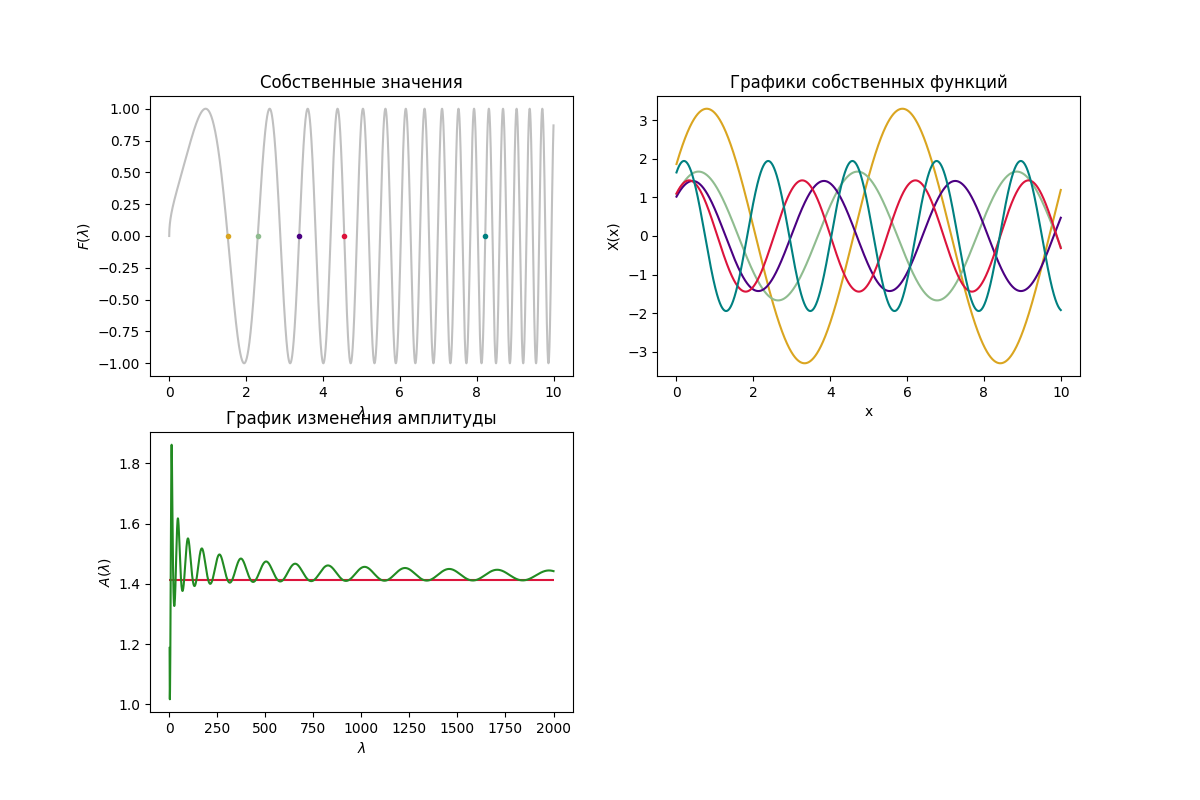
\includegraphics[scale=0.4]{UMF_PIC}}
	\caption{Численно построенные графики}
\end{figure}

На графиках собственных функций жёлтая линия соответствует собственному значению $\lambda_{1} = 1.52170$, зелёная - 
$\lambda_{2} = 2.30388$, фиолетовая - $\lambda_{3} = 3.38247$, красная -  $\lambda_{4} = 4.55452$ и синяя - $\lambda_{5} = 8.22286$.
Как видно из последнего графика, показывающего зависимость амплитуды колебаний от собственного значения, амплитуда колебаний при большом собственном значении оказывается примерно равным $\sqrt{\frac{2}{l}}$. Это же подтверждается и аналитически

\[ \lim\limits_{\lambda \to +\infty} \sqrt{\frac{1}{(1 + (\frac{\alpha}{\beta \sqrt{\lambda}})^2) (\frac{l}{2} - \frac{1}{2\sqrt{\lambda}} (\sin (2\sqrt{\lambda}l + \varphi) + \sin 2\varphi))}} =  \sqrt{\frac{2}{l}}. \]

\section{Основные свойства собственных чисел и собственных функций}
\begin{enumerate}
	\item Существует счётное число собственных значений $\lambda_1 < \lambda_2 < ... < \lambda_n < ... $, которым соответсвуют нетривиальные решения задачи - собственные функции $X_1 (x), X_2 (x), ..., X_n (x), ... $
	\item Собственные функции $X_n (x), X_m (x), n \neq m$ ортогональны между собой с весом $\rho (x)$ на отрезке $0 \leq x \leq l$.
\[ \int_{0}^{l} X_{n} (x) X_{m} (x) \rho (x) dx = 0, \quad (n \neq m). \]
	\item Если $X_n (x)$ является собственной функцией при собственном значении $\lambda_n$, то функция $A_n X_n (x)$ ($A_n$ - произвольная постоянная) также является собственной функцией для того же значения.
\end{enumerate}

Чтобы исключить неопределённость в выборе множителся, можно подчинить собственные функции требованию нормировки:
\[ ||X_n (x) ||^2 = \int_{0}^{l}  X^2_n (x) \rho (x) dx = 1. \] 
Тогда такие собственные функции образуют ортогональную и нормированную систему:
\begin{equation*}
	 \int_{0}^{l}  X_{n} (x) X_{m} (x) \rho (x) dx =  \begin{cases}
	0, n \neq m, \\
	1, n = m.
	\end{cases}
\end{equation*}

\section{Определения замкнтуности и полноты ортонормированной системы}
\textbf{Определение.} Ортонормированная система ${X_n (x)}$  называется \textit{замкнутой}, если каждая функция $f(x)$ может быть разложена в сходящийся в среднем ряд Фурье по функциям данной системы.
\[ \forall \varepsilon > 0 \quad \forall f \quad \exists f_1 f_2 ... f_n \quad | \quad ||\sum_{i = 1}^n f_i X_i (x) - f(x) || < \varepsilon  \]
\textbf{Определение.} Ортонормированная система ${X_n (x)}$  называется \textit{полной}, если не существует такой нетривиальной функции $f(x)$, что $\int_{0}^{l} f(x) X_n (x) \rho (x) dx = 0 \quad \forall n$.
\section{Определения поточечной и равномерной сходимости рядов Фурье. Теорема Стеклова о равномерной сходимости}
\textbf{Определение.} Ряд Фурье сходится поточечно , если
\[ \forall x \in [0, l] \quad \forall \varepsilon > 0 \quad \exists N_\varepsilon \quad \forall n > N \quad || \sum_{i = 1}^{n} f_i X_i (x) - f(x) || < \varepsilon\]
\textbf{Определение.} Ряд Фурье сходится равномерно, если
\[ \forall \varepsilon > 0 \quad \exists N_\varepsilon \quad \forall n > N \quad \forall x \in [0, l] \quad || \sum_{i = 1}^{n} f_i X_i (x) - f(x) || < \varepsilon\]
\textbf{Теорема В.А. Стеклова.} Произвольная, дважды непрерывно дифференцируемая функция $f(x)$, удовляетворяющая граничным условиям $f(0) = f(l) = 0$, разлагается в равномерно и абсолютно сходящийся ряд по собственным функциям $X_{n} (x)$:
\[ f(x) = \sum_{n = 1}^{\infty} f_n X_n (x) \quad f_n = \frac{1}{||X_n (x)||^2} \int_{0}^{l} f(x) X_n (x) \rho (x) dx \quad ||X_n (x) ||^2 = \int_{0}^{l}  X^2_n (x) \rho (x) dx \]

\chapter{Специальные функции}

\section{Функции Бесселя}
\subsection{Найти фундаментальную систему решений уравнения Бесселя $\nu-$го порядка}

Уравнение имеет вид:
\[ y'' + \frac{y'}{x} + (1 - \frac{\nu^2}{x^2}) y = 0, \]
где $\nu \in \mathbb{R}$ или $\nu \in \mathbb{C} \quad | \quad Re\nu < 0$.

Решение будем искать в виде:
\[ y = x^{\sigma} \sum_{n = 0}^{+\infty} a_{n} x^{n}, \quad a_{0} \neq 0, \]
поскольку уравнение имеет особенность в точке $x = 0$, $\sigma$ называется характеристическим показателем.

Подставим ряд в уравнение и соберём слагаемые при $x^{n + \sigma - 2}$:
\[ \sum_{n = 0}^{+\infty} (n + \sigma)(n + \sigma - 1)a_{n} x^{n + \sigma - 2} + (n+ \sigma)a_{n} x^{n + \sigma - 2} + a_{n} x^{n + \sigma} - \nu^2 a_{n} x^{n + \sigma - 2} = 0 \]
\[ \sum_{n = 0}^{+\infty} a_{n} x^{n + \sigma - 2} ((n + \sigma)^2 - \nu^2 + x^2) = \sum_{n = 0}^{+\infty} a_{n} x^{n + \sigma - 2} ((n + \sigma)^2 - \nu^2) + \sum_{n = 0}^{+\infty} a_{n} x^{n + \sigma} = 0\]

Приравняем к нулю коэффициенты при степенях $\sigma - 2$, $\sigma - 1$, ..., $n + \sigma - 2$:
\begin{equation*}
	\begin{cases}
		a_{0} (\sigma^2 - \nu^2) = 0 \\
		a_{1}((1 + \sigma)^2 - \nu^2) = 0 \\
		a_{2}((2 + \sigma)^2 - \nu^2) + a_{0} = 0 \\
		a_{3}((3 + \sigma)^2 - \nu^2) + a_{1} = 0 \\
		... \\
		a_{n}((n + \sigma)^2 - \nu^2) + a_{n - 2} = 0
	\end{cases}
\end{equation*}

Поскольку $a_{0} \neq 0$ по условию, то $\sigma^2 - \nu^2 = 0$ и $\sigma = \pm \nu$. Для второго уравнения системы с учётом предыдущей выкладки имеем:
\[ a_{1} (1 + 2\sigma + \sigma^2 - \nu^2) = a_{1} (1 + 2\sigma) = 0 \Rightarrow a_{1} = 0. \]

$\forall n > 1$ получим рекуррентную формулу для коэффициентов $a_{n}$:

\[ a_{n} (n + \sigma - \nu)(n + \sigma + \nu) + a_{n - 2} = 0 \]
\[ a_{n} = - \frac{a_{n - 2}}{(n + \sigma - \nu)(n + \sigma + \nu)} \]

Поскольку ранее было показано, что $a_{1} = 0$, то из рекуррентной формулы можно увидеть, что все $a_{2l + 1} = 0, \quad l > 0$.

При $\sigma = -\nu \in \mathbb{R}$ решение обращается в бесконечность в точке $x = 0$. Рассмотрим случай, когда $\sigma = \nu$, тогда для $a_{2l}, \quad l > 0$ рекуррентная формула примет вид:
\[ a_{2l} = - \frac{a_{2l - 2}}{2l(2l + 2\nu)} =  - \frac{a_{2l - 2}}{4l(l + \nu)} \]

Применим формулу последовательно, начиная с $a_{0}$:
\[ a_{2} = - \frac{a_{0}}{4(1 + \nu)} \]
\[ a_{4} = - \frac{a_{2}}{4*2(2 + \nu)} = \frac{a_{0}}{4^2 *1* 2 * (1 + \nu) * (2 + \nu)}\]
\[ a_{6} = - \frac{a_{4}}{4*3(3 + \nu)} = - \frac{a_{0}}{4^3 *1* 2 * 3 * (1 + \nu) * (2 + \nu) * (3 + \nu)}\]
\[ ... \]
\[ a_{2l} = (-1)^l \frac{a_{0}}{4^l * l! * (1 + \nu) * (2 + \nu) * ... * (l + \nu)} = -\frac{a_{0} \nu!}{4^l  l! (l + \nu)!}\]

Воспользуемся гамма-функцией и её свойствами. Выберем $a_{0} = \frac{1}{2^\nu \Gamma(\nu + 1)}$:
\[ a_{2l} = (-1)^l \frac{a_{0} \nu!}{4^l  l! (l + \nu)!} = (-1)^l \frac{a_{0} \Gamma(\nu + 1)}{2^{2l}  \Gamma(l + 1) \Gamma(l + \nu + 1)} = (-1)^l \frac{1}{2^{2l + \nu}  \Gamma(l + 1) \Gamma(l + \nu + 1)}\]

Если $\sigma = -\nu \neq -n$, где $n \in \mathbb{Z_{+}}$, то возьмём $a_{0} = \frac{1}{2^{-\nu}\Gamma(1 - \nu)}$ и получим:
\[ a_{2l} = (-1)^l \frac{1}{2^{2l - \nu} \Gamma(l + 1) \Gamma(l - \nu + 1)} \]

Полученные результаты подставим в ряд, который представляет собой решение уравнения.
\newline

\textbf{Определение.} $J_{\nu} (x) = \sum_{n = 0}^{+\infty} (-1)^n \frac{1}{\Gamma(n + 1) \Gamma(n + \nu + 1)} (\frac{x}{2})^{2n + \nu}$ называется \textit{функцией Бесселя первого рода $\nu-$го порядка}.
\newline

Это первое решение исходного уравнения, вторым решением является функция 
\[ J_{-\nu} (x) = \sum_{n = 0}^{+\infty} (-1)^n \frac{1}{\Gamma(n + 1) \Gamma(n - \nu + 1)} (\frac{x}{2})^{2n - \nu} \]

Эти решения линейно независимы, когда $\nu \notin \mathbb{Z}$.

Так как исходное уравнение является обыкновенным дифференциальным уравнением второго порядка, то его фундаментальная система решений состоит из двух линейно независимых решений.

Полученные ряды сходятся равномерно, так как член этих рядов можно оценить сверху $\frac{x^n}{n!}$, который является членом ряда, сумма которого равна $e^x$.

Таким образом решение $y(x) = C_1 J_{\nu} (x) + C_2 J_{-\nu} (x)$.
\newline

Запишем определитель Вронского этих двух функций:

\[ W(x) = \begin{vmatrix}	
			J_{\nu}(x) & J_{-\nu}(x) \\
			J'_{\nu}(x) & J'_{-\nu}(x)
		  \end{vmatrix} = \frac{2\sin \nu x}{\sqrt{x}}\]

Понятно, что когда $\nu$ не равно целому числу, тогда упомянутые функции будут линейно независимы. Если $\nu$ - целое, тогда определитель Вронского равен нулю, что говорит нам о линейной зависимости функций. 

Предположим, что $\nu = k$, тогда $\forall n = 0, 1, ..., k - 1$ слагаемые ряда  $J_{-k}(x)$ будут содержать в знаменателе гамма-функцию от отрицательного аргумента, тогда сама функция обращается в бесконечность и ряд имеет вид:
\[  J_{-k}(x) = \sum_{n = k}^{+\infty} (-1)^n \frac{1}{\Gamma(n + 1) \Gamma(n - k + 1)} (\frac{x}{2})^{2n - k} =   \sum_{m = 0}^{+\infty} \frac{ (-1)^{m + k}}{\Gamma(m + k + 1) \Gamma(m + 1)} (\frac{x}{2})^{2m + k} = (-1)^k J_k (x) \]

Установили линейную зависимость функций в этом случае.
\subsection{Получить рекуррентные формулы для функций Бесселя порядка $\nu$}

\textbf{Утверждение.} $\frac{d}{dx} \frac{J_{\nu}(x)}{x^{\nu}} = - \frac{J_{\nu + 1}(x)}{x^\nu}$
\newline

Доказательство.
\[ x^{\nu} \frac{d}{dx} \frac{J_{\nu}(x)}{x^{\nu}} = (\frac{x}{2})^{\nu} = \sum_{n = 1}^{+\infty} (-1)^n \frac{0.5 * n * (\frac{x}{2})^{2n - 1}}{n! \Gamma(n + \nu + 1)} = \sum_{n = 1}^{+\infty} \frac{(-1)^n}{\Gamma(n) \Gamma(n + \nu + 1)} (\frac{x}{2})^{2n + \nu - 1} = \]
\[ = -\sum_{l = 0}^{+\infty} \frac{(-1)^l}{\Gamma(l + 1)\Gamma(l + \nu + 1 + 1)} (\frac{x}{2})^{2l + \nu + 1} = - J_{\nu + 1}(x)\]

Поделим обе части равенства на $x^{\nu}$:
\[ \frac{d}{dx} \frac{J_{\nu}(x)}{x^{\nu}} = - \frac{J_{\nu + 1}(x)}{x^\nu} \]

\textbf{Утверждение.} $\frac{d}{dx} (x^{\nu} J_{\nu}(x)) = x^\nu J_{\nu - 1}(x)$
\newline

Доказательство.

\[ \frac{d(x^{\nu} J_{\nu}(x))}{dx} = \sum_{n = 0}^{+\infty} \frac{(-1)^k 2(k + \nu) * 0.5 * (\frac{x}{2})^{2(k + \nu) - 1}}{\Gamma(n + 1) \Gamma(n + \nu + 1)} = x^\nu \sum_{n = 0}^{+\infty} \frac{(-1)^n (n + \nu)}{(n + \nu) \Gamma(n + 1) \Gamma(n + \nu - 1 + 1)} (\frac{x}{2})^{2n + \nu - 1} = \]
\[ = x^\nu J_{\nu - 1}(x) \]

Теперь получим рекуррентные формулы, которые связывают $J_{\nu - 1}(x)$, $J_{\nu}(x)$, и $J_{\nu + 1}(x)$:
\begin{equation*}
	\begin{cases}
		\frac{\nu J_{\nu}(x)}{x} - J'_{\nu}(x) = J_{\nu + 1}(x) \\
		\frac{\nu J_{\nu}(x)}{x} + J'_{\nu}(x) = J_{\nu - 1}(x)
	\end{cases}
\end{equation*}
Сложим и вычтём уравнения системы друг из друга:
\begin{equation*}
	\begin{cases}
		J_{\nu + 1}(x) + J_{\nu - 1}(x) = \frac{2\nu}{x} J_{\nu}(x) \\
		J_{\nu + 1}(x) - J_{\nu - 1}(x) = -2 J'_{\nu}(x)
	\end{cases}
\end{equation*}

Таким образом:
\[  J_{\nu + 1}(x) = \frac{2\nu}{x} J_{\nu}(x) - J_{\nu - 1}(x) \]

\subsection{Вывести асимптотические формулы для функций Бесселя 1 и 2 рода}

\subsection{Построить графики функций Бесселя 1 и 2 рода для $\nu = 0.1$}
\begin{figure}[H]
	\center{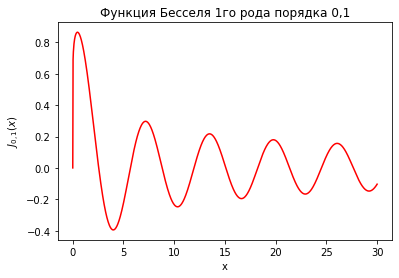
\includegraphics[scale=0.7]{BESSEL1}}
	\caption{График функции Бесселя первого рода порядка 0,1}
\end{figure}

\begin{figure}[H]
	\center{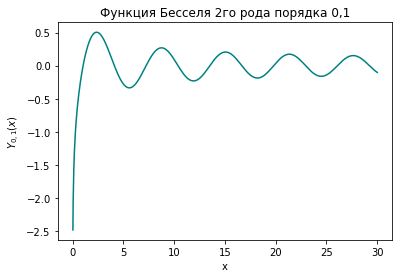
\includegraphics[scale=0.7]{BESSEL2}}
	\caption{График функции Бесселя второго рода порядка 0,1}
\end{figure}

\end{document}